%% ****** Start of file rsitemplate.tex ****** %
%%
%%   This file has been edited from the original source file.
%%	 The original file is part of the revtex4-1 package indicated below.
%%   Version 4.1 of 9 October 2009.
%%
%
% This is a template for producing documents for use with
% the REVTEX 4.1 document class and the RSI substyle.
%
% Copy this file to another name and then work on that file.
% That way, you always have this original template file to use.
\documentclass[aip,rsi,reprint]{revtex4-1} % for checking your page length
%\documentclass[aip,rsi,reprint,graphicx,draft]{revtex4-1} % for checking your page length
%\documentclass[aip,rsi,preprint,graphicx]{revtex4-1} % for review purposes
%\documentclass{aastex}

%\usepackage[warnundef]{jabbrv}

\usepackage{siunitx}
\DeclareSIUnit{\sqrthz}{\ensuremath{\sqrt{\text{\hertz}}}}

\usepackage{amsmath}
\usepackage{amsfonts}

\usepackage{graphicx}
\usepackage[caption=false]{subfig}
\usepackage{dcolumn}
\usepackage{multirow}
%\usepackage{caption}
%\usepackage{subcaption}

% \usepackage{aastex}
%\usepackage{natbib}
\usepackage{hyperref}

%% Work with illustrator *.ai files...
\DeclareGraphicsRule{.ai}{pdf}{.ai}{}
 

%% useful macros
\newcommand{\epar}{~||~} % add impedances in parallel
\newcommand{\CC}{{C\nolinebreak[4]\hspace{-.05em}\raisebox{.4ex}{\tiny\bf ++}}~}

%% ugh, should find better solution to this. ADS returns \prb, not recognized by revtex style...
\newcommand{\prb}{Phys. Rev. B}

\begin{document}

% Use the \preprint command to place your local institutional report number
% on the title page in preprint mode.
% Multiple \preprint commands are allowed.
%\preprint{}

\title{An ultra-low noise, high-voltage piezo driver}

% repeat the \author .. \affiliation  etc. as needed
% \email, \thanks, \homepage, \altaffiliation all apply to the current author.
% Explanatory text should go in the []'s,
% actual e-mail address or url should go in the {}'s for \email and \homepage.
% Please use the appropriate macro for the type of information

% \affiliation command applies to all authors since the last \affiliation command.
% The \affiliation command should follow the other information.

\author{N.C. Pisenti}
\email[]{npisenti@umd.edu}
\author{B.J. Reschovsky}
\author{D.S. Barker}
\author{A. Restelli}
\author{G.K. Campbell}
%\homepage[]{Your web page}
%\thanks{}
%\altaffiliation{}
\affiliation{Joint Quantum Institute, University of Maryland and National Institute of Standards and Technology}

% Collaboration name, if desired (requires use of superscriptaddress option in \documentclass).
% \noaffiliation is required (may also be used with the \author command).
%\collaboration{}
%\noaffiliation

\date{\today}

\begin{abstract}
We present an ultra-low noise, high voltage driver suited for use with piezoelectric actuators and other low-current applications.
The architecture leverages a commercially available, small-form-factor integrated circuit (IC) for generating high voltage outputs.
The IC uses a flyback configuration switching regulator to generate up to 250V in our design (but up to 1kV or more with small modification), and a high slew-rate op-amp capacitively coupled to the output compensates for the switching noise.
A low-voltage (\SI{\pm 10}{\volt}), high bandwidth modulation input is capable of summing small voltage corrections onto the output, making the driver well suited for use in closed-loop feedback applications.
\end{abstract}

\pacs{}% insert suggested PACS numbers in braces on next line

\maketitle %\maketitle must follow title, authors, abstract and \pacs

% Body of paper goes here. Use proper sectioning commands.
% References should be done using the \cite and \label commands
\section{Introduction}
\label{Sec:Introduction}

Many instrumentation applications in the modern laboratory require agile, low-noise voltage sources capable of supplying hundreds of volts or more.
For example, piezo-actuated mirrors and diffraction gratings play an important role in atomic physics experiments (used, e.g., in scanning Fabry-Per{\`o}t cavities and extended-cavity diode lasers), while avalanche photodiodes and photomultiplier tubes require large bias voltages for proper operation. 
In the realm of biophysics, electrokinetic separation methods such as free-flow or capillary electrophoresis require large electric field gradients, and the recent push to develop lab-on-a-chip devices could benefit from miniaturized high voltage sources~\cite{Kohlheyer2008a}. (ion traps? charge multiplier tubes?)

Often, laboratory devices are operated in a closed feedback loop, where small voltage changes on top of a large DC voltage are necessary to stabilize the output of a particular system.
For example, extended-cavity diode lasers can adjust their lasing frequency by changing the angle of a piezo-actuated diffraction grating that supplies optical feedback to the diode.
Commercially available piezoelectric drivers typically provide a modulation input for  such closed-loop applications, but the input voltage is either AC coupled to the output or gained such that it spans the entire voltage range of the device.
While this has certain advantages, many applications would benefit from an architecture that provides a unity gain, DC-coupled feedback path to the high voltage output. 
Such a device could make closed-loop systems less susceptible to noise contributions from the servo controller, which we often find in our laboratory to be the limiting factor in laser lock stability.

Traditionally, instrumentation electronics capable of supplying high voltages fall under one of two architectural umbrellas: DC-DC switching converters, and linear-type amplifiers.
While DC-DC converters are efficient and can work at very high voltages, they suffer from switching noise and limited control bandwidths.
Linear-type devices are typically constructed from a high-voltage operational amplifier (op-amp), powered either from a high voltage linear regulator or more typically from a secondary switching converter.
While the op-amp provides \SI{100}{\decibel} or more of power-supply noise rejection, high-voltage op-amps require substantially more power than an equivalent switching circuit and are more cumbersome to deploy in the laboratory.

Here, we present a hybrid architecture: the high voltage is generated by a galvanically isolated DC-DC converter (described in Sec.~\ref{Sec:DRV2700}), while a low-noise, high slew-rate op-amp removes noise at the output by modulating the {OUT--} node of the switching converter (see Sec.~\ref{Sec:LowNoiseStabilization}).
The op-amp additionally provides a low-gain, high-bandwidth modulation input for closed-loop feedback applications.
This architecture is able to achieve extremely low noise performance, draws very little current, and fits comfortably onto a small-footprint PCB.
Complete design files, including the schematic, bill of materials, and board layout, can be found on Github.~\footnote{\protect\url{https://github.com/JQIamo/hv-piezo-driver}}
% Mention other features?

%The high voltage setpoint is digitally controlled, and can be swept over \SI{200}{\volt} at \approx\SI{10}{\hertz}.


\section{Circuit Design}
\label{Sec:Circuit}

\begin{figure*}[t]
\includegraphics[width=\textwidth]{fig/DRV2700.ai}
\caption{Schematic of the high voltage stabilization.
The voltage HV is generated using a Texas Instruments DRV2700 high voltage driver in flyback configuration.
A fast, very high slew-rate op-amp senses the output voltage across $R_1$ and $R_2$, and servos it by modulating the node at ``HV floating gnd''.
The DC control signal for this op-amp is supplied by a digital-to-analog (DAC) converter, which is passed through a switchable low-pass filter. This allows for very heavy filtering of the DAC $1/f$ noise during steady-state operation, but the corner frequency can be increased if the output needs to be scanned more quickly.
The $\text{V}_{\text{DC}}$ gain is set by $\left(1+R_1/R_2\right)$, while the modulation gain is set by $-R_{\text{mod}}/R_1$.
The capacitor linking the floating ground node to the output allows the op-amp to remove residual switching noise and stabilize the DC output according to the transfer function given in Eq.~(\ref{Eq:FullTransferFunc}).
\label{Fig:PiezoCircuit}}
\end{figure*}

The design principles discussed below show how researchers might leverage the versatility of galvanically isolated switching regulators in a low-noise laboratory environment. 
Our design targets a \SI{250}{\volt} output, but straightforward modifications to the schematic make it possible to tailor the gain and output range to a specific application.
The entire electronics package fits comfortably into a 12HP eurocard rack module (with the high voltage section taking only a fraction of the PCB), and draws less than \SI{150}{\milli\ampere} at \SI{15}{\volt}.
%The full schematic, including Gerbers, a bill of materials, and layout design files, can be found on GitHub.~\footnote{\protect\url{https://github.com/JQIamo/hv-piezo-driver}}


\subsection{Flyback regulator}
\label{Sec:DRV2700}

The high voltage DC-DC converter used here is based on the Texas Instruments DRV2700 piezo driver\footnote{The identification of commercial products is for information only and does not imply recommendation or endorsement by the National Institute of Standards and Technology.}.
This single-chip integrated circuit (IC) can be operated as a boost converter to drive an on-chip differential amplifier up to \SI{100}{\volt}, or as a flyback converter up to \SI{1}{\kilo\volt} or more.
In flyback configuration, the internal-boost switch of the DRV2700 drives a step-up transformer.
When the switch closes, current begins to flow through the primary coil of the transformer and induces a corresponding voltage across the secondary coil.
In this state, the output diode is reverse-biased, and the capacitor ($\text{C}_{\text{HV}}$ in Fig.~\ref{Fig:PiezoCircuit}) holds its charge.
When the switch opens, the voltage across the secondary coil is inverted, putting the diode into conduction and charging the capacitor.
By changing the rate at which the switch is engaged, the DRV2700 is able to regulate a particular voltage across the galvanically isolated output (nodes $\text{GND}_\text{HV}$ and HV in Fig.~\ref{Fig:PiezoCircuit}).

The transformer (ATB3225, 1:10 step-up winding), diode, and RC feedback network are based on values suggested in the DRV2700 datasheet~\cite{DRV2700Datasheet,DRV2700EVMUserGuide}.
Internally, the DRV2700 boost controller tries to drive the FB node to \SI{1.3}{\volt}.
The op-amp U1 senses the voltage at nodes HV and $\text{GND}_\text{HV}$, and adjusts its output such that
\begin{align}
\label{Eq:U1Output}
\text{HV} - \text{GND}_{\text{HV}} &= G\cdot V_{\text{dc}}\,,
\end{align}
where the gain $G$ is set by the resistor ratio $R_3/R_4 \equiv R_5/R_6$.
This pseudo-differential feedback configuration ensures that, in the equilibrium given by Eq.~(\ref{Eq:U1Output}), the output of U1 is driven to \SI{0}{\volt}; the resistive divider $R_9$ and $R_{10}$ is then chosen such that $R_{10}/(R_9~||~R_{10}) = \SI{1.3}{\volt}/\SI{5}{\volt} \approx \num{0.26}$.
The capacitors $C_3$ and $C_4$ are chosen such that $C_3 = \SI{22}{\pico\farad}$ and
\begin{align}
\frac{C_4}{C_3} &= \frac{R_3}{R_4~||~R_7}
\end{align}
as suggested by the datasheet, and $R_6 = R_7 = R_8$.
In our lab, we implement a gain $G\approx 50$ ($R_3 = R_5 = \SI{499}{\kilo\ohm}$; $R_4 = R_{6-8} = \SI{10}{\kilo\ohm}$) such that a \SI{5}{\volt} digital-to-analog converter (DAC) controlling the node $\text{V}_\text{DC}$ can span \SI{250}{\volt} at the output.

The output of the flyback regulator is passed through a four-pole, low-pass RC filter.
The corner frequency $f_c \approx \SI{3}{\kilo\hertz}$ is chosen to be high enough that a slow ($\approx \SI{10}{\hertz}$) rail-to-rail triangle ramp can be applied by the DAC at $\text{V}_\text{DC}$ (for, e.g., sweeping over a spectroscopy resonance), but low enough that the $\approx \SI{100}{\kilo\hertz}$ switching noise is substantially attenuated.
Additional capacitors on both the HV and $\text{GND}_{\text{HV}}$ resistor networks shunt high frequency noise to ground.

\subsection{Low-noise stabilization}
\label{Sec:LowNoiseStabilization}

The low-noise stabilization circuit is crucial to the performance of the design, as it is responsible for removing noise at the output of the flyback converter.
To accomplish this, a high slew-rate op-amp (Texas Instruments LM7171, \SI[per-mode=symbol]{4100}{\volt\per\micro\second}) drives the galvanically isolated ground node of the flyback converter (see U2 in Fig.~\ref{Fig:PiezoCircuit}).
This op-amp enforces the HV output voltage
\begin{align}
\text{V}_\text{HV} &= \left(1 + \frac{R_1}{R_2~||~R_\text{mod}}\right) \text{V}_\text{DC} -
\left(\frac{R_\text{mod}}{R_1}\right) \text{V}_\text{mod}\,.
\label{Eq:FullTransferFunc}
\end{align}
We choose $R_1,\,R_\text{mod} = \SI{1}{\mega\ohm}$, $R_2 = \SI{20.5}{\kilo\ohm}$ such that the DC gain is $\approx 50$ and the modulation gain $\text{V}_\text{HV}/\text{V}_\text{mod}$ is unity.
Depending on the application, other gain configurations would work equally well provided the non-inverting gain of U2 closely matches the gain of the flyback regulator (since they derive from the same control voltage).
Ultimately, the op-amp U2 sets the operating voltage of the output (referenced to true circuit ground) while the flyback converter regulates the high voltage relative to the pseudoground node $\text{GND}_\text{HV}$.
Because the output of the flyback regulator is galvanically isolated, U2 is free to control $\text{GND}_\text{HV}$. 
At low frequencies, this amounts to changing the ``zero-volt'' reference for the flyback regulator, while at high frequencies the capacitor $\text{C}_\text{HV}$ provides a low-impedance pathway to the HV output.
In this manner, U2 is simultaneously able to servo residual switching noise and provide a DC-coupled, high-bandwidth modulation of the output.

As a final note, it is worth mentioning that the choice of component for resistors $R_1$ and $R_2$ is crucial for the low-noise performance of the system, because this resistive divider is responsible for accurately sensing the voltage $\text{V}_\text{HV}$; noise introduced by these resistors cannot be corrected by the op-amp, and thus appears directly at the output.
Resistors are fundamentally limited by Johnson noise, in which thermal fluctuations contribute to a white noise power spectrum given by $\sqrt{k_B T R}$.(Cite art of electronics?)\cite{Horowitz1989a}
However, resistors also exhibit $1/f$ current noise caused by equilibrium fluctuations of the resistance~\cite{Clarke1974a,Voss1976a}.
The magnitude of this ``excess noise'' is highly dependent on the resistor composition, and varies from manufacturer to manufacturer.
Seifert, et. al.~\cite{Seifert2009a} characterized $1/f$ noise in a variety of resistors, and found that the Vishay TNPW \SI{0.1}{\percent}-series resistors showed a noise spectrum almost consistent with Johnson noise down to \SI{1}{\hertz}.
A previous iteration of this design used Panasonic ERJ-8ENF resistors (1206, \SI{1}{\percent}), and we noticed substantial low-frequency noise correlated with varying strain on the PCB.
This is consistent with the findings in~\cite{Seifert2009a}, which showed this Panasonic series to exhibit voltage noise two orders of magnitude larger than the TNPW series at \SI{1}{\hertz}.
The final board design utilizes three TNPW \SI{0.1}{\percent} 0603 resistors in series for both R1 and R2.

\subsection{Digital control and auxiliary design features}
\label{Sec:DigControlAuxDesign}

The DC setpoint is controlled by a low-noise digital-to-analog converter (DAC).
This has several advantages: digital control enhances setpoint repeatability, and makes it easy to integrate with a wide variety of computerized control electronics.
The DAC itself is controlled by an onboard microcontroller, which also interacts with the frontpanel control switches, encoders, and LCD display.
The entire circuit is designed to fit in a standard Eurocard rack, which supplies power at $\pm\SI{15}{\volt}$ and contains a backplane with analog lines to communicate with other modules (e.g., to implement a current feed-forward for laser diodes, see description below).
The backplane also contains a secondary microcontroller, which can be addressed over TCP/IP.
This vastly expands the conceivable control scenarios. For example, in our lab we implement a slow-feedback lock of two ECDL repumping lasers to a wavemeter.
LabView code on the computer attached to the wavemeter computes an error signal and corrective control voltage, which can then be passed over our internal network to the piezo driver to correct for frequency drifts in the laser.
Other similar schemes are possible, enabling complete remote control of the laser electronics.

In addition to software-defined control via the backplane, frontpanel control is provided by a rotary encoder/push button, and a single SPDT switch.
The encoder/push button provide menu navigation, and the switch toggles between DC and scanning operation.
However, other user interfaces can easily be designed to work with the existing hardware.
Arduino-based code written in \CC defines the entire software interaction, and can be modified depending on the needs of the researcher.

A voltage proportional to the output (sensed at the inverting node of U2) is buffered and connected to a monitor BNC on the frontpanel and a GPIO line on the backplane.
In our lab, this GPIO line is fed to a low-noise current controller (based on the design in~\cite{Erickson2008a}) to implement a current feed-forward.
An optional analog voltage from the backplane can also be summed with the modulation voltage supplied via BNC on the frontpanel to generate $\text{V}_{\text{mod}}$.
This may be useful, e.g., with servo controllers that reside in the same rack as the other control electronics.

Finally, the high voltage output is interlocked with a signal on the back plane (which can optionally be over-ridden by placing a jumper); this allows easy integration into existing laboratory interlock schemes, if desired.
For more details, see the design files and documentation on Github~\cite{DesignFiles}.



\subsection{Noise Analysis}
\label{Sec:NoiseAnalysis}

\begin{figure}[t]
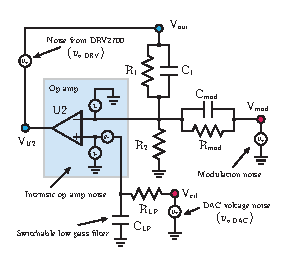
\includegraphics[width=\columnwidth]{fig/NoiseModel.ai}
\caption{Noise model (see text). In reality, the capacitor labeled $Z_\text{LP}$ is comprised of a \SI{47}{\nano\farad} capacitor in parallel with a switchable \SI{10}{\micro\farad} capacitor, such that the corner frequency of the filter can be changed depending on the mode of operation. The $\text{R}_\text{on}$ resistance of the switch introduces a zero in the transfer function at $\approx\SI{23}{\kilo\hertz}$, which has negligible effect on the computed RMS noise. \label{Fig:NoiseModel}}
\end{figure}

\begin{figure}[t]
\subfloat{
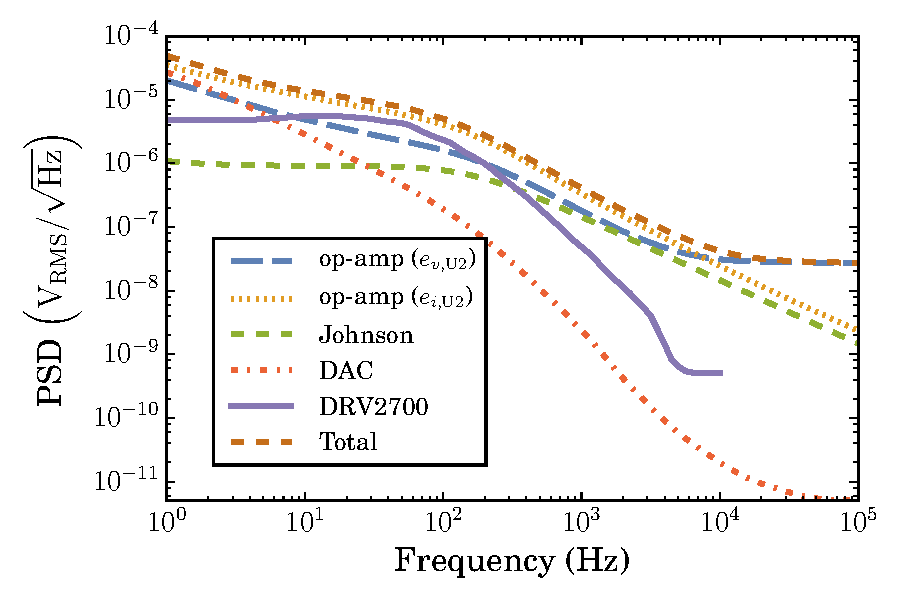
\includegraphics[width=\columnwidth]{fig/NoiseContrib.pdf}
}

\subfloat{
\centering
\begin{tabular*}{0.95\columnwidth}{@{\extracolsep{\fill}} lcc}
\hline\hline
\rule{0pt}{2.5ex}\multirow{2}{*}{Noise source} & RMS Voltage & RMS Voltage \\
& (\SI{1}{\hertz}~--~\SI{10}{\hertz})\rule[-1ex]{0pt}{1ex} & (\SI{10}{\hertz}~--~\SI{100}{\kilo\hertz})\rule[-1ex]{0pt}{1ex} \\
\hline
\rule{0pt}{2ex}$e_n$ (op-amp)  & \SI{26}{\micro\volt} & \SI{27}{\micro\volt}      \\
$i_n$ (op-amp)  &            \SI{49}{\micro\volt}     & \SI{59}{\micro\volt}      \\
DAC             &             \SI{22}{\micro\volt}    & \SI{7}{\micro\volt}       \\
Johnson-Nyquist &             \SI{3}{\micro\volt}    & \SI{31}{\micro\volt}        \\ 
\hline
\rule{0pt}{2ex}\textbf{total (calculated)} & \SI{60}{\micro\volt} & \SI{73}{\micro\volt}  \\
\hline\hline
\end{tabular*}
}
\caption{Noise Contributions (color online). Plotted are the noise contributions from each source in our model, along with the total calculated noise. Power spectral density is referred to the high voltage output, and the table shows the integrated RMS noise due to each noise source in different frequency bands. The total RMS noise (summed in quadrature) over the entire \SI{1}{\hertz}~--~\SI{100}{\kilo\hertz} range is calculated to be \SI{94}{\micro\volt}. \label{Fig:NoisePlot}}
\end{figure}

We analyze the noise performance of the circuit according to the model shown in Fig.~\ref{Fig:NoiseModel}, where noise spectral densities are calculated at the node $\text{V}_\text{HV}$.
A summary of each noise contribution (op-amp, DAC, Johnson-Nyquist, external modulation input) is shown in Fig.~\ref{Fig:NoisePlot}, along with the cumulative root-mean-square (RMS) nose estimates in different frequency bands.
% We also discuss, given our choice of op-amp, the noise rejection ratio from the DRV2700 flyback regulator.
% -- not sure about how to do this... could just report the measured value.

To treat the intrinsic op-amp noise contributions, we first compute the noise gain ($NG$) for this amplifier configuration according to
\begin{align}
\label{Eq:NG}
NG(s) &= 1 + \frac{Z_1}{R_2 \epar Z_{\text{mod}}}\,,
\end{align}
where we've defined the equivalent impedances $Z_1 = R_1/(1+R_1 C_1 s)$ and $Z_{\text{mod}} = R_{\text{mod}}/(1+R_{\text{mod}} C_{\text{mod}} s)$, and $s = i\omega$ is the frequency in the Laplace domain.
By design, we've chosen $Z_1 \equiv Z_{\text{mod}}$ such that the signal gain from the node $\text{V}_{\text{mod}}$ is unity.
This reduces Eq.~(\ref{Eq:NG}) to
\begin{align}
\label{Eq:RedNG}
NG(s) &= 2 + \frac{Z_1}{R_2}\,.
\end{align}

The op-amp noise is parametrized by two noise contributions: $e_n$, the input voltage noise power spectral density (PSD), and $i_n$, the input current noise PSD.
For the LM7171, $e_n = \SI[per-mode=symbol]{14}{\nano\volt\per\sqrthz}$ and $i_n = \SI[per-mode=symbol]{1.5}{\pico\ampere\per\sqrthz}$ at $\SI{10}{\kilo\hertz}$, with a $1/f$ noise character below this frequency~\cite{LM7171Datasheet}.
The voltage noise is summed in at the non-inverting input, while the current noise is present at both inputs.
To convert $i_n$ to an equivalent voltage noise $e_n$, we multiply by the impedances $Z_n$, $Z_p$ seen by the inverting and non-inverting nodes, respectively.
These are calculated as
\begin{align}
\begin{split}
\label{Eq:ZnZp}
Z_n &= Z_1 \epar Z_{\text{mod}} \epar  R_2   = \frac{Z_1}{2} \epar R_2 \\
Z_p &= R_{\text{LP}}  \big|\big|\frac{1}{s~C_{\text{LP}}}
\end{split}
\end{align}
The total noise contribution of the op-amp (referenced to the output) is
\begin{align}
\label{Eq:OpAmpNoise}
e_{n,\text{op-amp}} &= NG(s)\sqrt{e_n^2 + (Z_n i_n)^2 + (Z_p i_n)^2}
\end{align}

We now calculate the noise contribution of the DAC.
The noise signal gain from the node $\text{V}_{\text{DC}}$ is given by
\begin{align}
\begin{split}
\label{Eq:Gdc}
G_{\text{DC}} &= \left(\frac{Z_\text{LP}}{R_\text{LP} + Z_\text{LP}}\right)\left(1+\frac{Z_1}{R_2\epar Z_{\text{mod}}}\right) \\
&= \left(\frac{Z_\text{LP}}{R_\text{LP} + Z_\text{LP}}\right)NG(s)\,,
\end{split}
\end{align}
where the first term represents the contribution to the transfer function from the switchable low-pass filter (discussed above).
The DAC voltage noise contribution is then simply $e_{n,\text{DAC}} = G_{\text{DC}} v_{n,\text{DAC}}$. 
The DAC used in our design (Analog devices, AD5663R) has a white noise floor of \SI[per-mode=symbol]{100}{\nano\volt\per\sqrthz} with an $\approx\SI{1}{\kilo\hertz}$ corner frequency.
Without the addition of the low-pass filter after $\text{V}_\text{DC}$, this DAC would dominate both the low- and high-frequency noise performance of the circuit.
However, we are instead dominated by Johnson noise at intermediate to high frequencies, and the op-amp's intrinsic current noise at lower frequencies.
Both of these contributions could potentially be suppressed by using lower resistances $R_1, R_\text{mod}$, however one must be careful about power and current limitations when dealing with such high voltages.
Each noise source is tabulated and plotted in Fig.~\ref{Fig:NoisePlot}.


\section{Results}
\label{Sec:Results}
Here, we show the measured performance of the high-voltage piezo driver.
In Fig.~\ref{Fig:PSD}, we plot the noise power spectral density measured at several different output voltages.
These traces were taken on an SR780 spectrum analyzer, with the piezo output coupled through a \SI{0.5}{\hertz} high-pass filter. 
At \SI{100}{\volt}, the integrated noise ($\SI{1}{\hertz} - \SI{100}{\kilo\hertz}$) was measured to be $\SI{80}{\micro\volt}_\text{RMS}$ ($\SI{138}{\micro\volt}_\text{RMS}$, $\SI{101}{\micro\volt}_\text{RMS}$ for \SI{50}{\volt}, \SI{200}{\volt} outputs). 
This matches well with the expected total RMS noise calculated in Section~\ref{Sec:NoiseAnalysis}.

\begin{figure}[hb]
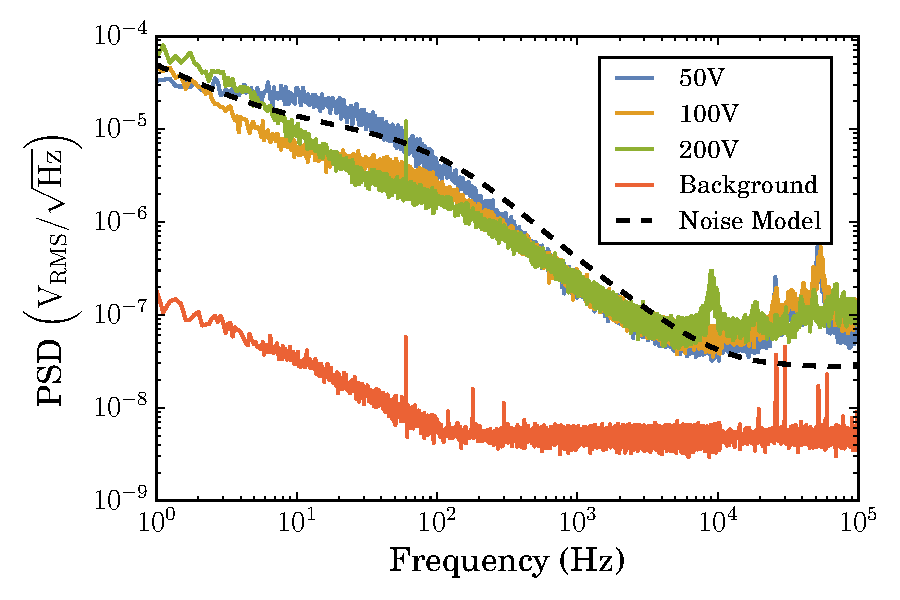
\includegraphics[width=\columnwidth]{fig/VoltagePSD.pdf}
\caption{Voltage power spectral density at various output voltages. The integrated RMS voltage noise ($\SI{1}{\hertz} - \SI{100}{\kilo\hertz}$) is $\{138, 80, 101\}~\si{\micro\volt}$ measured at  $\{50, 100, 200\}~\si{\volt}$. \label{Fig:PSD}}
\end{figure}

Figure~\ref{Fig:TimeDomain} shows the performance at both short- and long-time scales.
At long times, voltage fluctuations on the order of a few \si{\milli\volt} can be observed.
This is due generically to $1/f$ noise, but also correlates with the external temperature.
A cross-correlation between measured temperature and output voltage fluctuation yields an effective temperature coefficient of \SI[per-mode=symbol]{-24}{ppm\per\celsius} at \SI{100}{\volt}.
The short-term trace was taken on a PicoScope~5442B (ac-coupled, \SI{100}{\volt} output).
Points are colored based on their normally distributed statistical probability, and thus give a visual estimation of the RMS width.

\begin{figure}[h]
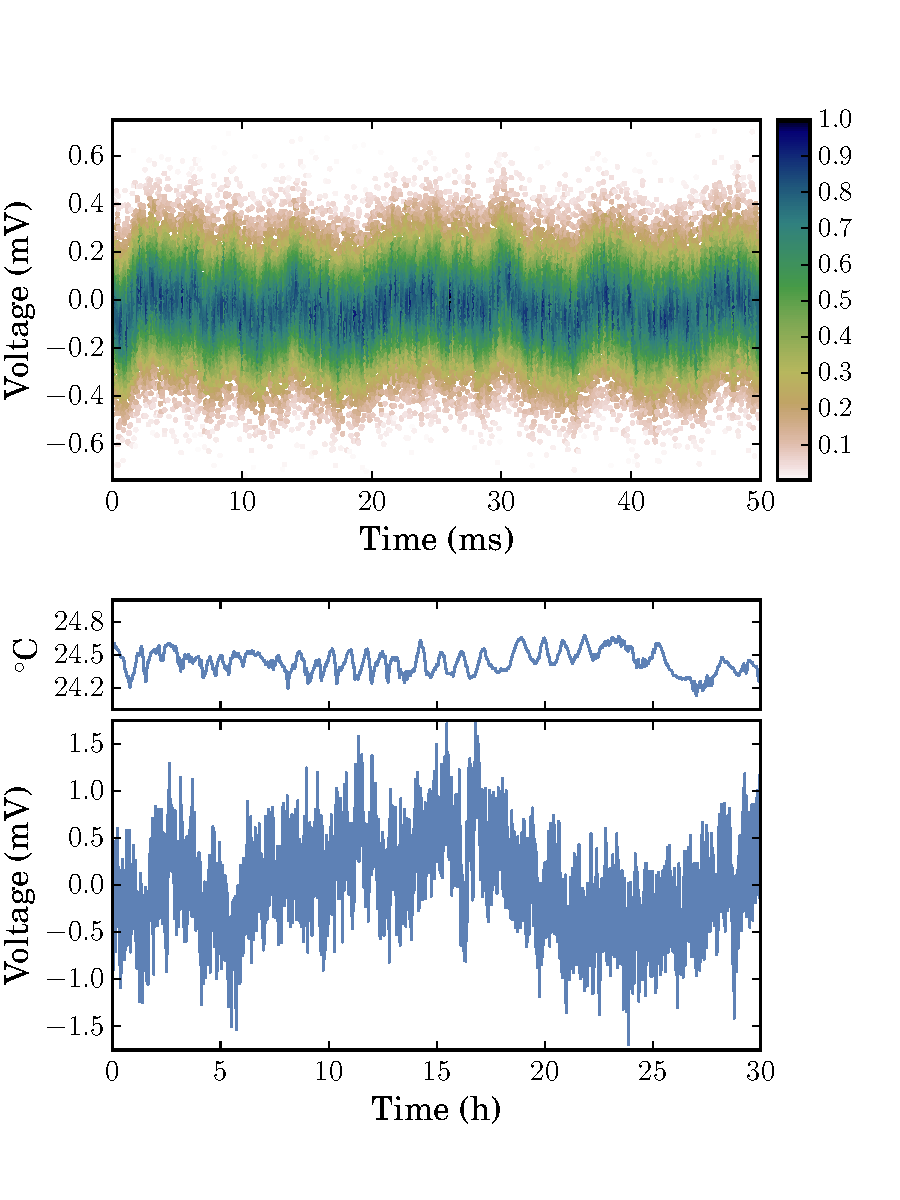
\includegraphics[width=\columnwidth]{fig/TimeDomain.pdf}
\caption{Time-domain traces of the high voltage output (\SI{100}{\volt}). Top: short-time scatterplot  (AC coupled). Points are colored based on the Gaussian spread in acquired voltages, thus indicating the RMS width of the trace. Bottom: long-term trace, measured on a Keithly~2010 digital multimeter. A~\SI{100}{\volt} DC offset is subtracted from the plotted values. The top trace shows the lab temperature during the same time period.\label{Fig:TimeDomain}}
\end{figure}

Finally, Figure~\ref{Fig:TransferFunc} shows the measured frequency response under different load conditions. The unloaded bandwidth is as high as a few megahertz, while a \SI{1}{\micro\farad} capacitive load can still be driven at $\approx\SI{100}{\kilo\hertz}$. 
Several mechanical resonances can be seen with a \SI{700}{\nano\farad} piezoelectric load, as might be expected.
In a laboratory setting, these resonances can be mitigated by using a digital feedback controller with notch filters tuned to match the exact resonance frequencies observed in the system\cite{Ryou2016a}, thereby extending the usable bandwidth out to $\approx\SI{100}{\kilo\hertz}$.
\begin{figure}[h]
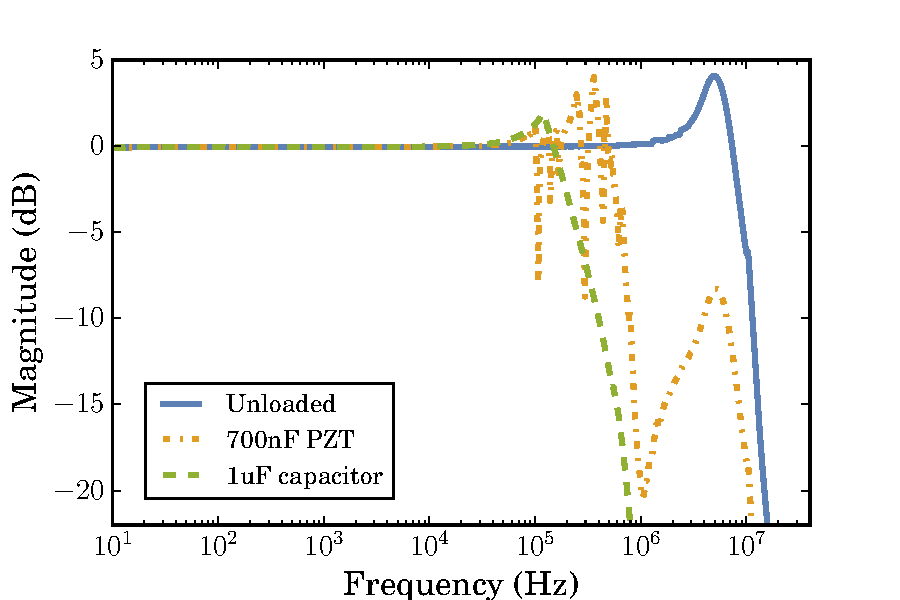
\includegraphics[width=\columnwidth]{fig/PiezoModulationTransfer.pdf}
\caption{Modulation input transfer function. Green trace shows the response with a ThorLabs piezoelectric actuator {(PN~AE0505D08F)}; the mechanical resonances above $\approx\SI{50}{\kilo\hertz}$ are clearly visible. The red trace shows the response under a \SI{1}{\micro\farad} purely capacitive load. Loaded response bandwidth is $\approx\SI{100}{\kilo\hertz}$, while unloaded the bandwidth is $\approx\SI{1}{\mega\hertz}$.\label{Fig:TransferFunc}}
\end{figure}

\section{Conclusion}
\label{Sec:Conclusion}

We have designed, built, and characterized a high-voltage piezoelectric circuit optimized for use in a modern atomic physics laboratory.
It is based on a flyback configuration switching regulator, but is able to achieve very low noise performance by active stabilization from a high slew-rate op-amp.
This hybrid architecture makes it small and easy to deploy in a variety of situations, without requiring an external, bulky high-voltage power supply.
The design principles discussed here can be adapted to fit the exact application, and all design files are freely available on GitHub for others to use and modify.

The authors would like to thank Z. Smith for useful discussions.

This work was partially supported by ONR, and the NSF through the PFC at the JQI.

%
%\section{Other...}
%\begin{itemize}
%\item $1/f \rightarrow$ white noise corner frequency
%\item white noise spectral density
%\item RMS noise (0.1 - 10 Hz; 10 Hz - 10 kHz, or something similar) -- use SRS voltage preamp?
%\item How effective is the LM7171 at reducing switching noise? look at FFT power before final filter resistor, and at output of op amp (dBc spec)
%\item compare noise to predicted values
%\item longterm trace on kiethly -- across voltage divider at output? Monitor vs temperature? -- need to find low Tc resistors, at least.
%\item see what dependence is on power source -- eg, JQI power supply vs lab supply vs very quiet voltage regulator?
%\item current draw -- display in some ``bottom line'' specs table?
%\item bandwidth measurements -- full scale triangle ramp, small signal bandwidth -- discuss limitations on this (eg, also versus different piezo loads)
%\item Lock a laser, show RMS noise fluct vs. old piezo?
%\item compare to SC100 toptica controller? even if just internally.
%\end{itemize}


% If in two-column mode, this environment will change to single-column format so that long equations can be displayed.
% Use only when necessary.
%\begin{widetext}
%$$\mbox{put long equation here}$$
%\end{widetext}

% Figures should be put into the text as floats.
% Use the graphics or graphicx packages (distributed with LaTeX2e). EPSFig is no longer fully supported.
% See the LaTeX Graphics Companion by Michel Goosens, Sebastian Rahtz, and Frank Mittelbach for examples.
%
% Here is an example of the general form of a figure:
% Fill in the caption in the braces of the \caption{} command.
% Put the label that you will use with \ref{} command in the braces of the \label{} command.
%
% \begin{figure}
% \includegraphics{}% % Important NOTE: Please make certain your figures do not include local directory paths. ex. "c:\file\sub\fig1.eps"
% \caption{\label{}}%
% \end{figure}

% Tables may be be put in the text as floats.
% Here is an example of the general form of a table:
% Fill in the caption in the braces of the \caption{} command. Put the label
% that you will use with \ref{} command in the braces of the \label{} command.
% Insert the column specifiers (l, r, c, d, etc.) in the empty braces of the
% \begin{tabular}{} command.
%
% \begin{table}
% \caption{\label{} }
% \begin{tabular}{}
% \end{tabular}
% \end{table}

% If you have acknowledgments, this puts in the proper section head.
%\begin{acknowledgments}
% Put your acknowledgments here.
%\end{acknowledgments}

% Create the reference section using BibTeX:
%\bibliographystyle{jabbrv_abbr}
\bibliography{piezobib}
% Run this once to generate your BBL file. Then copy the contents of your BBL file into your main latex file, commenting out "\bibliography"

\end{document}
%
% ****** End of file aiptemplate.tex ******
